\documentclass{article}

\usepackage{geometry}
\usepackage{amsmath}
\usepackage{graphicx, eso-pic}
\usepackage{listings}
\usepackage{hyperref}
\usepackage{multicol}
\usepackage{fancyhdr}
\pagestyle{fancy}
\fancyhf{}
\hypersetup{ colorlinks=true, linkcolor=black, filecolor=magenta, urlcolor=cyan}
\geometry{ a4paper, total={170mm,257mm}, top=10mm, right=20mm, bottom=20mm, left=20mm}
\setlength{\parindent}{0pt}
\setlength{\parskip}{0.3em}
\renewcommand{\headrulewidth}{0pt}

\rfoot{\thepage}
\fancyhf{} % sets both header and footer to nothing
\renewcommand{\headrulewidth}{0pt}
\lfoot{\textbf{Seleksi IEEEXtreme 17.0 ITB}}
\pagenumbering{gobble}

\fancyfoot[CE,CO]{\thepage}
\lstset{
    basicstyle=\ttfamily\small,
    columns=fixed,
    extendedchars=true,
    breaklines=true,
    tabsize=2,
    prebreak=\raisebox{0ex}[0ex][0ex]{\ensuremath{\hookleftarrow}},
    frame=none,
    showtabs=false,
    showspaces=false,
    showstringspaces=false,
    prebreak={},
    keywordstyle=\color[rgb]{0.627,0.126,0.941},
    commentstyle=\color[rgb]{0.133,0.545,0.133},
    stringstyle=\color[rgb]{01,0,0},
    captionpos=t,
    escapeinside={(\%}{\%)}
}

\begin{document}

\begin{center}

    
    \section*{Caffeine Fighter} % ganti judul soal

    \begin{tabular}{ | c c | }
        \hline
        Batas Waktu  & 1s \\    % jangan lupa ganti time limit
        Batas Memori & 256MB \\  % jangan lupa ganti memory limit
        \hline
    \end{tabular}
\end{center}

\subsection*{Deskripsi}

Kirima Syaro sedang mengikuti festival tahunan di sekolahnya. Sekolah Syaro memiliki salah satu acara rutin yang ada pada festival tersebut yaitu lari marathon. Pada acara marathon terdapat N buah pos dinomori dari 1 sampai N dimana terdapat jalan-jalan yang menyambungkan antar pos dengan jarak K meter. Tujuan dari acara marathon kali ini adalah untuk sampai ke pos tujuan dimulai dari pos mulai dengan waktu sesingkat mungkin.\\

Syaro tidak percaya diri akan kemampuan larinya sehingga Ia hanya bertujuan untuk sampai ke pos tujuan dalam maksimal X menit. Namun karena Syaro tidak pandai berlari, Ia hanya bisa berjalan secepat 1 meter per detik. Beruntung ada kakak kelas favorit Syaro yaitu Rize. Rize membawakan Syaro minuman favoritnya yaitu kopi. Dengan zat kafein yang terdapat pada kopi membuat kecepatan lari Syaro meningkat sebanyak 1 meter per detik setiap meminum satu gelas kopi.\\

Karena meminum terlalu banyak kopi tidak baik untuk kesehatan, Syaro ingin Ia memenuhi target waktu sampainya namun dengan meminum kopi seminimum mungkin. Diketahui juga bahwa ketika sudah mencapai sebuah pos, peserta lari akan memilih pos selanjutnya untuk dikunjungi dan hanya boleh mulai berlari ketika detik pada waktu adalah xx:00 (penjelasan lebih detail ada pada contoh). Bantu Syaro untuk mengetahui jumlah kopi minimum yang harus Ia minum agar bisa sampai ke pos tujuan dalam waktu X menit. Perhatikan juga bahwa bisa saja mustahil bagi Syaro untuk sampai pos tujuan dalam waktu X menit, untuk kasus ini keluarkan nilai -1.\\

Keterangan batasan antar pos:
\begin{enumerate}
    \item dipastikan pos awal dan pos tujuan tidak sama
    \item untuk jalan antar pos tidak mungkin ada 2 jalan yang dengan pos awal dan pos tujuan yang sama (no multi edge)
    \item tidak ada jalan antar pos dengan pos awal dan pos tujuan yang sama (no self loop)
    \item dipastikan ada jalan dari pos awal ke pos tujuan
    \item untuk sebuah jalan antar pos bersifat bolak-balik
\end{enumerate}

\subsection*{Format Masukan}

Baris pertama terdiri dari lima bilangan bulat positif $N, M, X, A, B (1 \leq N \leq 10^5, N-1 \leq M \leq 10^5, 1 \leq X \leq 10^9, 1 \leq A,B \leq N, A \neq B)$, yang merupakan banyaknya pos, banyak jalan antar pos, target waktu sampai Syaro, pos awal dan pos tujuan acara marathon kali ini.\\

M baris selanjutnya terdiri dari tiga bilangan bulat positif $u, v, K (1 \leq u, v \leq N, 1 \leq K \leq 10^9)$, yang menyatakan terdapat jalan antar pos u dan pos v, dan jarak jalan antar pos tersebut.

\subsection*{Format Keluaran}

Keluarkan sebuah bilangan bulat positif yang merupakan jumlah kopi minimum yang perlu Syaro minimum untuk memenuhi target waktunya, atau keluarkan -1 apabila Syaro tidak bisa sampai kurang dari waktu yang ditargetkan.

\begin{multicols}{2}
\subsection*{Contoh Masukan}
\begin{lstlisting}
4 3 4 1 2
4 3 247
2 3 352
1 4 300
\end{lstlisting}
\columnbreak
\subsection*{Contoh Keluaran}
\begin{lstlisting}
4
\end{lstlisting}
\vfill
\null
\end{multicols}

\subsection*{Penjelasan}
Berikut adalah ilustrasi peta acara marathon yang diikuti Syaro.\\
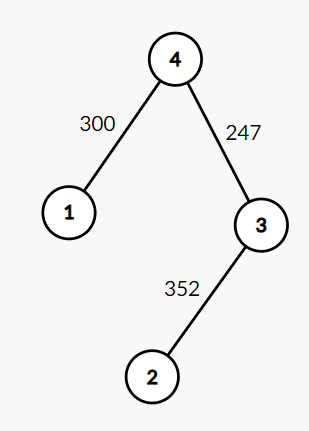
\includegraphics[scale=0.6]{graph}\\
Pada kasus ini, Syaro memulai larinya pada pos 1 dan ingin sampai ke pos tujuan yaitu pos 2 dengan target waktu maksimal 4 menit.\\

Berikut adalah beberapa ilustrasi perjalanan Syaro dengan berbagai situasi banyaknya kopi yang ia minum, dengan asumsi ia memulai larinya pada pukul 00:00.\\
Apabila Syaro tidak meminum kopi, maka kecepatan larinya adalah 1 meter per detik.\\
Ketika ia sampai ke pos 4 dari pos 1 pada pukul 05:00, ia bisa langsung melanjutkan perjalanannya.\\
Ketika ia sampai ke pos 3 dari pos 4 pada pukul 09:07, ia baru bisa melanjutkan perjalanan pada pukul 10:00.\\
Ketika ia sampai ke pos 2 dari pos 3 pada pukul 15:52.\\
Jadi Syaro akan sampai pada pos 2 kurang dari 16 menit apabila ia tidak meminum kopi.\\

Apabila Syaro meminum 6 kopi, maka kecepatan larinya adalah 7 meter per detik.\\
Apabila Syaro tidak meminum kopi, maka kecepatan larinya adalah 1 meter per detik.\\
Ketika ia sampai ke pos 4 dari pos 1 pada pukul 00:43, ia baru bisa melanjutkan perjalanan pada pukul 01:00.\\
Ketika ia sampai ke pos 3 dari pos 4 pada pukul 01:36, ia baru bisa melanjutkan perjalanan pada pukul 02:00.\\
Ketika ia sampai ke pos 2 dari pos 3 pada pukul 02:51.\\
Jadi Syaro akan sampai pada pos 2 kurang dari 3 menit apabila ia tidak meminum kopi.\\

Dari seluruh kemungkinan, jumlah kopi minimum yang perlu Syaro minum agar ia bisa sampai ke pos 2 dalam waktu maksimal 4 menit adalah 4 kopi.


\end{document}